\documentclass[12pt]{article}
\usepackage[utf8]{inputenc}
\newcommand\preamble{
    \usepackage[italian]{babel}
    \usepackage{geometry}
    \usepackage{amsmath}
    \usepackage{amssymb}
    \usepackage{graphicx}
    \usepackage{ulem}
    \usepackage[table, dvipsnames]{xcolor}
    \usepackage{tikz}
    \usepackage{qtree}
    \usepackage{spverbatim}
    \usepackage{listings}
    \usepackage{hyperref}

    \usetikzlibrary{er, positioning}
    \usetikzlibrary{arrows}

    \tikzset {multi attribute/.style={attribute,double distance=1.5pt}}
    \tikzset {derived attribute/.style={attribute,dashed}}
    \tikzset {total/.style={double distance=1.5pt}}
    %\tikzset {every entity/.style={ draw=orange,fill=orange!20}}
    %\tikzset {every attribute/.style={draw=purple,fill=purple!20}}
    %\tikzset {every relationship/.style={draw=green,fill=green!20}}

    \geometry{margin=2cm}
    \let\olditemize\itemize
    \renewcommand\itemize{\olditemize\setlength\itemsep{0em}}
    \graphicspath{{../Immagini/}}

    \author{Lorenzo Vaccarecci}

    \definecolor{codegreen}{rgb}{0,0.6,0}
    \definecolor{codegray}{rgb}{0.5,0.5,0.5}
    \definecolor{codepurple}{rgb}{0.58,0,0.82}
    \definecolor{backcolour}{rgb}{0.95,0.95,0.92}

    \lstdefinestyle{mystyle}{
        backgroundcolor=\color{backcolour},   
        commentstyle=\color{codegreen},
        keywordstyle=\color{magenta},
        numberstyle=\tiny\color{codegray},
        stringstyle=\color{codepurple},
        basicstyle=\ttfamily\footnotesize,
        breakatwhitespace=false,         
        breaklines=true,                 
        captionpos=b,                    
        keepspaces=true,                 
        numbers=left,                    
        numbersep=5pt,                  
        showspaces=false,                
        showstringspaces=false,
        showtabs=false,                  
        tabsize=2
    }

    \lstset{style=mystyle}

    \hypersetup{
        colorlinks=true,
        linkcolor=blue,
        filecolor=magenta,      
        urlcolor=blue,
        pdfpagemode=FullScreen,
    }

    \urlstyle{same}
}
\newcommand {\key}[1]{\underline{#1}}
\newcommand {\question}[1]{\textit{#1}\\}
\newcommand {\important}[1]{\textcolor{red}{#1}}
\newcommand {\remark}[1]{\textcolor{Cyan}{#1}}
\preamble

\title{Controllo dell'Accesso}
\date{10 Maggio 2024}

\begin{document}
\maketitle
\section{Introduzione}
Il problema è che \textbf{non tutti gli utenti possono eseguire le stesse operazioni} (\textit{es. gestore e cliente}). Lo scopo del controllo dell'accesso è quello di \textbf{limitare e controllare} le operazioni degli utenti e \textbf{prevenire} azioni che potrebbero compromettere la correttezza e la sicurezza del sistema. Le operazioni vengono catturate prima di essere eseguite.
\section{Politiche di sicurezza}
\begin{itemize}
    \item \remark{Regole e principi}: per la protezione delle informazioni
    \item \remark{Insieme di direttive ad alto livello}
\end{itemize}
\textit{Es. "le valutazioni dei film possono essere viste solo dal responsabile della videoteca"}.\\
Tre entità principali:
\begin{itemize}
    \item \important{Oggetti}: sono le risorse a cui vogliamo garantire protezione (le tabelle)
    \item \important{Soggetti}: sono le entità (gli utenti)
    \item \important{Privilegi}: descrivono quali operazioni possono essere eseguite dai soggetti sugli oggetti
\end{itemize}
\section{Controllo degli Accessi in SQL}
\begin{itemize}
    \item \important{Sistema chiuso}: un accesso è concesso solo se è stato esplicitamente permesso
    \item \important{Amministrazione decentralizzata} (mediante \textbf{ownership}): l'utente che crea una relazione, riceve privilegi di controllo su di essa e può concedere o revocare privilegi
    \item \important{\texttt{GRANT}}: se un privilegio è concesso con grant option l'utente che lo riceve può non solo esercitare il privilegio, ma anche concederlo ad altri
    \item \important{\texttt{REVOKE}}: toglie i privilegi a uno o più utenti
\end{itemize}
\subsection{\texttt{GRANT}}
L'inserimento di una nuova autorizzazione avviene tramite il comando \texttt{GRANT}:
\begin{lstlisting}[language=SQL]
    GRANT {<lista privilegi> | ALL PRIVILEGES}
    ON <nome oggetto>
    TO {<lista utenti> | <lista ruoli> | PUBLIC}
    [WITH GRANT OPTION];
\end{lstlisting}
La lista dei privilegi è composta da: \texttt{SELECT}, \texttt{INSERT}, \texttt{UPDATE}, \texttt{DELETE}, ecc.\\ 
\texttt{WITH GRANT OPTION} (opzionale) consente la delega dell'amministrazione dei privilegi.
Alla creazione di una risorsa, il creatore riceve automaticamente tutti i privilegi su di essa quindi \textbf{i comandi di \texttt{GRANT}} corrispondenti vengono \textbf{eseguiti automaticamente} dal sistema.
Possiamo concedere il privilegio anche su singole colonne.
\href{https://2023.aulaweb.unige.it/pluginfile.php/352748/mod_resource/content/4/03A-controlloAccesso-23-24.pdf}{Esempi di \texttt{GRANT} (p.20)}.
\subsection{\texttt{REVOKE}}
La revoca di privilegi avviene tramite il comando \texttt{REVOKE}:
\begin{lstlisting}[language=SQL]
    REVOKE [GRANT OPTION FOR] <lista privilegi>
    ON <nome oggetto>
    FROM <lista utenti>
    [CASCADE | RESTRICT];
\end{lstlisting}
La clausola opzionale \texttt{GRANT OPTION FOR}, se presente, revoca il privilegio di concedere il privilegio ad altri utenti. \textbf{Un utente può revocare solo i privilegi concessi da lui.}
\section{Rappresentazione delle autorizzazioni}
In modo astratto le informazioni contenute nei cataloghi possono essere rappresentate in astratto come un insieme di grafi (\important{grafi delle autorizzazioni}). \important{Esiste un grafo per ogni privilegio $p$ su una certa tabella}. Un grafo delle interrogazioni per il privilegio sulla tabella $R$ contiene:
\begin{center}
    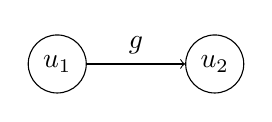
\begin{tikzpicture}[node distance={20mm}, main/.style = {draw, circle}] 
        \node[main] (1) {$u_{1}$};
        \node[main] (2) [right of = 1] {$u_{2}$}; 
        \draw[->] (1) -- node[above] {$g$} (2);
    \end{tikzpicture}
\end{center} 
Un nodo per ogni utente che ha il privilegio $p$ sulla tabella $R$. L'arco uscente da $u_{1}$ verso $u_{2}$ indica che $u_{1}$ ha concesso il privilegio a $u_{2}$ ed è etichettato $g$ se è concesso con \texttt{GRANT OPTION}.
\begin{center}
    \includegraphics[scale=0.4]{esempioautorizzazioni.png}
\end{center}
Un comando di \texttt{GRANT} può essere eseguito parzialmente in alcuni casi:
\begin{center}
    \includegraphics[scale=0.4]{esempiograntparziale.png}
\end{center}
Il comando \texttt{REVOKE}:
\begin{center}
    \includegraphics[scale=0.4]{esempiorevoke.png}
\end{center}
\texttt{RESTRICT}: non elimina altri nodi oltre quello designato\\
\texttt{CASCADE}: elimina anche tutti i nodi che dipendono da quello designato, quindi se un nodo è puntato da due nodi, viene eliminato solo l'arco che parte dal nodo chiamante (però i figli vengono eliminati).
\begin{center}
    \includegraphics[scale=0.4]{esempiorevokecascade.png}
\end{center}
Se non si specifica niente, il comportamento di default è \texttt{RESTRICT}.
\section{Ruoli}
I ruoli sono funzioni svolte in ambito di un'organizzazione. \important{Gli utenti sono abilitati a ricoprire uno o più ruoli}. I privilegi possono essere concessi anche ai ruoli, le autorizzazioni specificate per un ruolo sono quelle necessarie per esercitare le funzioni connesse al ruolo stesso. Semplificano l'attribuzione dei privilegi ai soggetti.
\begin{lstlisting}[language=SQL]
    CREATE ROLE <nome ruolo>;
    DROP ROLE <nome ruolo>;
    SET ROLE <nome ruolo>; -- Associazione dimanica di un ruolo all'utente della sessione attiva
\end{lstlisting}
Nel comando \texttt{GRANT} mettiamo
\begin{lstlisting}[language=SQL]
    GRANT <lista ruoli>
    TO {<lista utenti> | PUBLIC}
    [WITH ADMIN OPTION]; -- Analogo a GRANT OPTION
\end{lstlisting}
E' possibile dare una gerarchia ai ruoli:
\begin{lstlisting}[language=SQL]
    GRANT <ruolo_figlio> 
    TO <ruolo_padre>;
\end{lstlisting}
I privilegi del figlio sono acquisiti dal padre ma non viceversa.
\\\textbf{Esempio:}
\begin{lstlisting}[language=SQL]
    CREATE ROLE direttoreVideoteca;
    CREATE ROLE commesso;

    GRANT SELECT ON film TO commesso;
    GRANT INSERT, DELETE ON film TO direttoreVideoteca;
    GRANT commesso TO direttoreVideoteca;
\end{lstlisting}
Di solito prima si danno i privilegi(specifici) ai figli e poi al padre.
\subsection{REVOKE}
\begin{lstlisting}[language=SQL]
    REVOKE [ADMIN OPTION FOR]
    <lista ruoli>
    FROM <lista utenti>
\end{lstlisting}
\section{Controllo dell'accesso basato sul contenuto}
\subsection{Autorizzazione su Viste}
Le viste consentono di realizzare il così detto
\important{controllo dell'accesso in base al contenuto}. Permettono di concedere anche \important{privilegi statistici} (es. una vista che computa il numero di noleggi effettuati da ogni cliente e concedere all'utente l'accesso alla vista invece che alla tabella).\\
\question{Chi può creare una vista?}
\remark{Gli utenti che hanno il privilegio di \texttt{SELECT} su tutte le tabelle utilizzate dalla vista.}\\
\question{Il proprietario della vista quali privilegi può esercitare sulla vista?}
Bisogna considerare:
\begin{itemize}
    \item Le autorizzazioni sulle tabelle coinvolte ($P1$)
    \item \href{https://2023.aulaweb.unige.it/pluginfile.php/352757/mod_resource/content/3/LinguaggioSQLParte4DatiDerivati-23-24.pdf}{Regole per formare le autorizzazioni $P2$ (p. 26)}
\end{itemize}
\remark{Il proprietario ha i privilegi che ha sono l'intersezione tra $P1$ e $P2$}.
\end{document}